\label{ch:proced}
The method applied here is a combination of three concepts described in chapter \ref{ch:calcPES}.
It is based on the time-independent DO formalism where the electronic structure is computed by means of the OTRSH density functional.
%The FEF is obtained by the finite/infinite element method as described in chapter \ref{ch:fem}.
This combination represents a novelty of this work, sinse the DO approach has not yet been used together with OTRSH TDDFT, which is most suited among different functionals for PES calculations.
The last but not least is the application of the finite and infinite element methods to obtain FEFs.
To the best of my knowledge this method is used to solve such quantum-mechanical problem for the first time.

In the first section of this chapter, the computation of the wave functions of initial (unionised) and final (ionised) states as well as the genaral procedure used to compute the DOs is described.
Thereafter, in section \ref{sec:grid} the setup of the finite/infinite element system is explained which is implemented in the program \prog{FreeWilly} \cite{FreeWilly} in the framework of this thesis.
This program is used to compute the free electron function as well as the dipole transition matrix elements.

\section{Bound State Functions}
The DO formalism as it is described in section \ref{ch:do} can be used with any electronic structure method which can predict excited state energies and wave functions such as configuration interaction \cite{ci1}, generalised active space configuration interaction \cite{bauch1}, equation-of-motion coupled cluster \cite{CAPccEOM,eomCCdo}, complete and restricted self-consistent field \cite{MAgg,GrellKuehn,asscf1,asscf2} or TDDFT as given in Table \ref{tab:PEScat}.
In this work, DFT is used for ground state calculations and its time-dependent counterpart, TDDFT, to compute excited state energies.
The DFT formalism which is briefly introduced in the sections \ref{ch:dft} and \ref{ch:tddft} has shown to be accurate and computationally efficient.
%In this work the calculations are done using a locally modified version of the program package \prog{NWChem} \cite{nwchem} where a more verbose output enables the reconstruction of all molecular orbitals and thus the computation of the DOs.

\subsection{Ground State Density}
\label{ch:dft}
The DFT is formally based on the Hohenberg-Kohn theorems \cite{HohenbergKohn} which state that the ground-state electron density $\rho(\vec{r})$ determines the potential in the SE and with this also the wave function.
Moreover, the energy of the ground state can be found variationally.
Thus, the electron density contains all information needed and the computation of the $N$-electron wave function can be omitted.
Since the Hohenberg-Kohn theorems do not point out a way how to determine the electron density without knowing the wave function, usually the Kohn-Sham scheme \cite{KohnSham} is used.
In this framework, the electrons are described as non-interacting particles in a respective pseudo-potential that is constructed such that the Kohn-Sham density coincides with the real one.
Since the particles do not interact with each other, the Kohn-Sham orbitals $\Psi_j(\vec{r})$ can be obtaind from the one-particle SE
\begin{equation}
\left( -\frac 12  \nabla^2 + V_\text{eff}(\vec{r}) \right) \Psi_j(\vec{r})=\epsilon_j \Psi_j(\vec{r}),
\end{equation}
where $\epsilon_j$ is the energy of the respective Kohn-Sham orbital $\Psi(\vec{r})$ and the effective potential 
\begin{equation} \label{eq:dftPot}
V_\text{eff}(\vec{r})=V_\text{ext}(\vec{r})+ \int \frac{\rho(\vec{r}')}{|\vec{r}-\vec{r}'|} d\vec{r}' + V_\text{xc}(\vec{r})
\end{equation}
can be separated into the external potential $V_\text{ext}(\vec{r})$, which consists of the attractive nuclear ESP and external fields, the electrostatic interaction of the particles whith a charge density $\rho(\vec{r})=\sum_i |\Psi_i|^2$ and the exchange-correlation potential $V_\text{xc}(\vec{r})$ which contains the complexity of the interelectronic interaction \cite{baerRSH}.
The exchange-correlation potential $V_\text{xc}(\vec{r})$ contains, besides contributions from exchange and correlation, also correction for the error in kinetic energy present due to the fact that the Kohn-Sham wave functions differ from the real orbitals \cite{Holthausen}.

The exact exchange-correlation potential $V_\text{xc}(\vec{r})$ is not known, giving rise to different variants of approximate functionals, each suited for particular problems and applications.
However, usually the exchange-correlation term is split into an exchange and a correlation parts for which separate approximations are used.
The exact exchange potential acting on an orbital $\Psi_i(\vec{r})$ has the form
\begin{equation} \label{eq:HF_exch}
V_{x;j}(\vec{r})\Psi_i(\vec{r}) =-\int \frac{\Psi_j^\dagger(\vec{r}') \Psi_i(\vec{r}')}{\left|\vec{r}-\vec{r'}\right|} d\vec{r}' \Psi_j(\vec{r})
\end{equation}
and thus is non-local \cite{Holthausen}.
The term ``exact'' indicates here that using the exchange potential \eq{eq:HF_exch} the self-interaction error of the Coulomb term (\textit{i.e} the second term in equation \eq{eq:dftPot}) cancels out completely.
%The term exact exchange is under %energy thus corresponds the term $E_{x}=\sum_{i<j}\int \Psi_i^\dagger(\vec{r}) V_{x;j}(\vec{r}) \Psi_i(\vec{r}) d\vec{r}$  respectively.
In DFT, usually the exchange energy is approximated as a local functional of the density and its derivative, leading to the so-called local density approximation and gradient corrected functionals \cite{baerRSH}.
The Becke \cite{blyp} exchange-functional used in this work has the form
\begin{equation} \label{eq:blypXC}
E_x=\frac 32 \left(\frac{3}{4\pi}\right)^\frac 13 \sum_\sigma \int \rho_\sigma(\vec{r})^\frac 43 d^3\vec{r} 
-\beta \sum_\sigma \int \rho_\sigma(\vec{r})^\frac 43 \frac{x_\sigma(\vec{r})^2}{1+6\beta x_\sigma \text{sinh}^{-1}( x_\sigma (\vec{r}))} d^3\vec{r},
\end{equation}
where the first summand corresponds to the local density approximation and the second is a semi-empirical gradient correction, $\sigma$ denotes the spin orientations and $x_\sigma(\vec{r})=\nicefrac{|\nabla \rho_\sigma(\vec{r})|}{\rho_\sigma^\frac 43}$. 
The gradient correction in this functional is constructed such that the asymptotic behaviour of the exchange energy and electron density follow
\begin{align} \label{eq:dftAsympt}
  \lim_{r\rightarrow\infty} E_x^\sigma(\vec{r}) & =-\frac{1}{|\vec{r}|} \\
  \lim_{r\rightarrow\infty} \rho(\vec{r}) & =e^{-a_\sigma |\vec{r}|}
\end{align}
with $a_\sigma$ is a constant related to the ionisation potential of the system under study \cite{blyp}.
The prefactor of the gradient correction, $\beta$, was determined by fitting to experiments for noble gas atoms and is set to be $\beta=0.0042$\,a.u. \cite{blyp}.
However, this parameter is not universal and errors in the asymtotic behaviour \eq{eq:dftAsympt} can occur for general systems.

%Finally, the correlation energy is defined as the difference between the sum of the previously discussed terms and the correct energy.
The correlation potential finally is defined as the functional derivative of the correlation energy with respect to the electron density $V_c(\vec{r})=\frac{\partial E_c[\rho]}{\partial\rho(\vec{r})}$.
In the case of the LYP-correlation energy functional applied here, the correlation energy is fitted to experimental data using two parameters using various closed and open shell systems \cite{lyp}.

\subsection{Properties of Excited States}
\label{ch:tddft}
Since the gound-state density fully specifies the system's Hamiltonian, it contains information on the excited staets which can be extracted from the response of the density to the periodic external fields via the time-dependent DFT (TDDFT) which is based on the Runge-Gro\ss\, theorem \cite{RungeGross}.
Commonly, when referring to TDDFT, the respective linear-response scheme is meant \cite{dreuw}.
It employs the configuration interaction philosophy, where an excited state wave function $|\Psi^\text{exc}\rangle$ is written as
\begin{equation} \label{eq:excCI}
|\Psi^\text{exc}\rangle=\sum_{ia} c_{ia} |\Psi_i^a\rangle.
\end{equation}
Here $|\Psi_i^a\rangle$ are Slater determinants in which the electron is excited from $i$-th occupied orbital to the virtual orbital $a$ and $c_{ia}$ are coefficients whose absolute squares sum up to one.


It is a first order perturbation expansion and can be used to obtain the energies and wave functions of excited states using the so-called Casida-equation \cite{casida}
\begin{equation} \label{eq:casida}
\begin{bmatrix} \mat{A} & \mat{B} \\ \mat{B}^\dagger & \mat{A}^\dagger\end{bmatrix}
\begin{bmatrix} \vec{X} \\ \vec{Y} \end{bmatrix} =
\omega \begin{bmatrix} \mat{1} & \mat{0} \\ \mat{0} & -\mat{1}\end{bmatrix}
\begin{bmatrix} \vec{X} \\ \vec{Y} \end{bmatrix},
\end{equation}
where the matrix elements are
\begin{align}
\mat{A}_{ia,jb}& =\delta_{ij}\delta_{ab}(\varepsilon_a-\varepsilon_i)+ 
\int \int d\vec{r} d\vec{r}'\frac{ \Psi_i(\vec{r}) \Psi_a(\vec{r})  \Psi_j(\vec{r}') \Psi_b(\vec{r}')- 
\Psi_i(\vec{r}) \Psi_j(\vec{r}) \Psi_a(\vec{r}') \Psi_b(\vec{r}')}{|\vec{r}-\vec{r}'|} ,\\
\mat{B}_{ia,jb}& = \int \int d\vec{r} d\vec{r}'\frac{\Psi_i(\vec{r}) \Psi_a(\vec{r})  \Psi_b(\vec{r}') \Psi_j(\vec{r}')- 
\Psi_i(\vec{r}) \Psi_b(\vec{r})  \Psi_a(\vec{r}') \Psi_j(\vec{r}')}{|\vec{r}-\vec{r}'|}.
\end{align}
Here $i,j$ denote occupied and $a,b$ are virtual states and $\mat{1}$ is the unity matrix, $\varepsilon_\alpha$ are the energies of the Kohn-Sham orbitals $\Psi_\alpha(\vec{r})$ \cite{dreuw}.
%The indices $i,j$ and $a,b$ denote occupied and virtual orbitals with binding energy $\varepsilon_i, \varepsilon_a$ respectively \cite{dreuw}.
The Casida equation (\ref{eq:casida}) is an non-hermitian eigenvalue problem whose eigenvalues $\omega$ correspond to the transition energies and the eigenvectors contain the transition coefficients $c_{ia}$ from \eq{eq:excCI}.
The different blocks in equation (\ref{eq:casida}) have different physical interpretation.
Because of the negative sign of the transition energy, the $\vec{Y}$ counterpart of the eigenvector can be assigned to de-excitations from virtual orbitals.
For the excited states it corresponds to orbital relaxation \cite{dreuw}.
Since the matrix $\mat{B}$ contains usually only small elements, it is often set to zero which is refferred to as Tamm-Dancoff approximation and reduces the original equation to a hermitian equation of half dimensionality with only small loss in accuracy \cite{casida}.

\subsection{Optimally-Tuned Range-Separated Hybrid Functional}
\label{ch:otrsh}
%One main issue concerned with the DFT-formalism is that the approximate exchange functional decays exponentially instead of $\frac 1r$ and $\frac{1}{r^4}$ for the exchange and correlation terms respectively \cite{Bokareva}. \textcolor{red}{But the Becke functional should have fixed this!?}
One main disadvantage of the DFT-formalism is that the approximate exchange functional lead to wrong asymptotic behaviour of the electron density.
The local density approximation leads to an exponential decay instead of $\frac 1r$ and $\frac{1}{r^4}$ for the exchange and correlation terms respectively \cite{Bokareva} which is improved significantly with gradient-corrected functionals but usually still yields spuirous behaviour \cite{baerRSH}.
This issue is known as self-interaction error because the approximate exchange potentials do not eliminate the interaction of an electron with itself at large interaction distances.
This is opposite to the exact exchange potential \eq{eq:HF_exch}, where such elimination is strictly fulfilled.
This wrong behaviour affects the obtained wave functions and thus the orbital energies and implicitly influences other system properties \cite{OT-RSH}.

To reduce this error, so-called range-separated hybrid functionals are used, in which the DFT exchange term as, \textit{e.g.}, the Becke functional (\ref{eq:blypXC}) is used for small interelectronic distances only, while at larger distances, where correlation effects are not that important, the Hartree-Fock exact exchange (\ref{eq:HF_exch}) is used \cite{LC-tddft}.
The interchange between the exact and approximate exchange functionals is done by some smooth function, for instance
\begin{equation}
   \frac 1r = \underbrace{\frac{\alpha +\beta \text{erf}(\omega r)}{r}}_{\text{exact exchange}} +\underbrace{\frac{1-\alpha-\beta \text{erf}(\omega r)}{r}}_{\text{DFT exchange}},
\end{equation}
where $\alpha+\beta=1$ and $\omega$ are parameters to be chosen.
These parameters are density- and thus system dependent.
Besides taking the standard parameters that are fitted for a set of test systems, \textit{ab initio} schemes for choosing $\alpha$ and $\omega$ are available which are referred to as optimally-tuned range-separated hybrid (OTRSH) density functionals.
Using such an approach, the Koopmans' theorem can be ensured by minimising following functional with respect to $\alpha$ and $\omega$ \cite{Bokareva}
\begin{equation}\label{eq:J_ao}
   J(\alpha_\text{opt},\omega_\text{opt})=\text{min}_{\alpha, \omega} \left\{ |E_N(\alpha,\omega)-E_{N-1}(\alpha,\omega)-\varepsilon_\text{HOMO}| \right\},
\end{equation}
where $E_N$ and $E_{N-1}$ are the ground state DFT energies of the $N$- and $N-1$-electron states and $\varepsilon_\text{HOMO}$ corresponds to the binding energy of the highest occupied molecular orbital (HOMO) of the $N$-electron system.
Such a procedure improves the asymptotic behaviour of the density and with this the orbital energies.
The latter is important especially for the photoelectron spectra and usually improves the calculated ionisation potentials.
However, this procedure is in general providing several optimal ($\alpha$,$\omega$) pairs.

Another property to be ensured during the optimisation is the derivative discontinuity \cite{derdis,sanchez,Autschbach}.
The exact exchange-correlation energy should be a straight line when varying the number of electrons from $N$ to $N-1$.
The slope of that line corresponds to the binding energy of the respective electron that is removed and thus is discontinuous at integer numbers of electrons.
The approximate exchange-correlation functionals, however, usually do not fulfill this condition having curvelinear dependence of energy with a wrong derivative jump or no discontinuity at all.
The criterion for $E_\text{xc}(N)$ to be a straight line is used additionally to choose the best pair ($\alpha$,$\omega$) for the particular system.

In this work, for the optimization procedure the Gaussian package \prog{G09} \cite{g09} was used with the 6-31G(d) \cite{6-31g,6-31gd} basis set and the LC-BLYP exchange-correlation functional \cite{lcblyp}. 
The ground state DFT calculation and optimisation of geometries have been conducted with a locally modified version of \prog{NWChem} \cite{nwchem}, employing the basis set def2-TZVP \cite{def2tzvp} without symmetry restrictions.

The application of the functional \eq{eq:J_ao} to the benzene molecule for different parameters $\alpha$ and $\omega$ results in a deviation from Koopman's theorem as illustrated in the left panel in Figure \ref{fig:Benzotrsh}.
This behaviour is typical for this functional when varying the parameters $\alpha$ and $\omega$ for different systems.
%As the Figure \ref{fig:Benzotrsh} illustrates, leads the imposition of Koopmans' theorem not to a unique set of parameters.
%Instead, a larger constant exact exchange $\alpha$ can be compensated by a smaller $\omega$, \textit{i.e.} the non-constant contributions are added for a larger radius.
%TODO Please do some corrections to the figure specified in the paper version of this section 
\begin{figure}
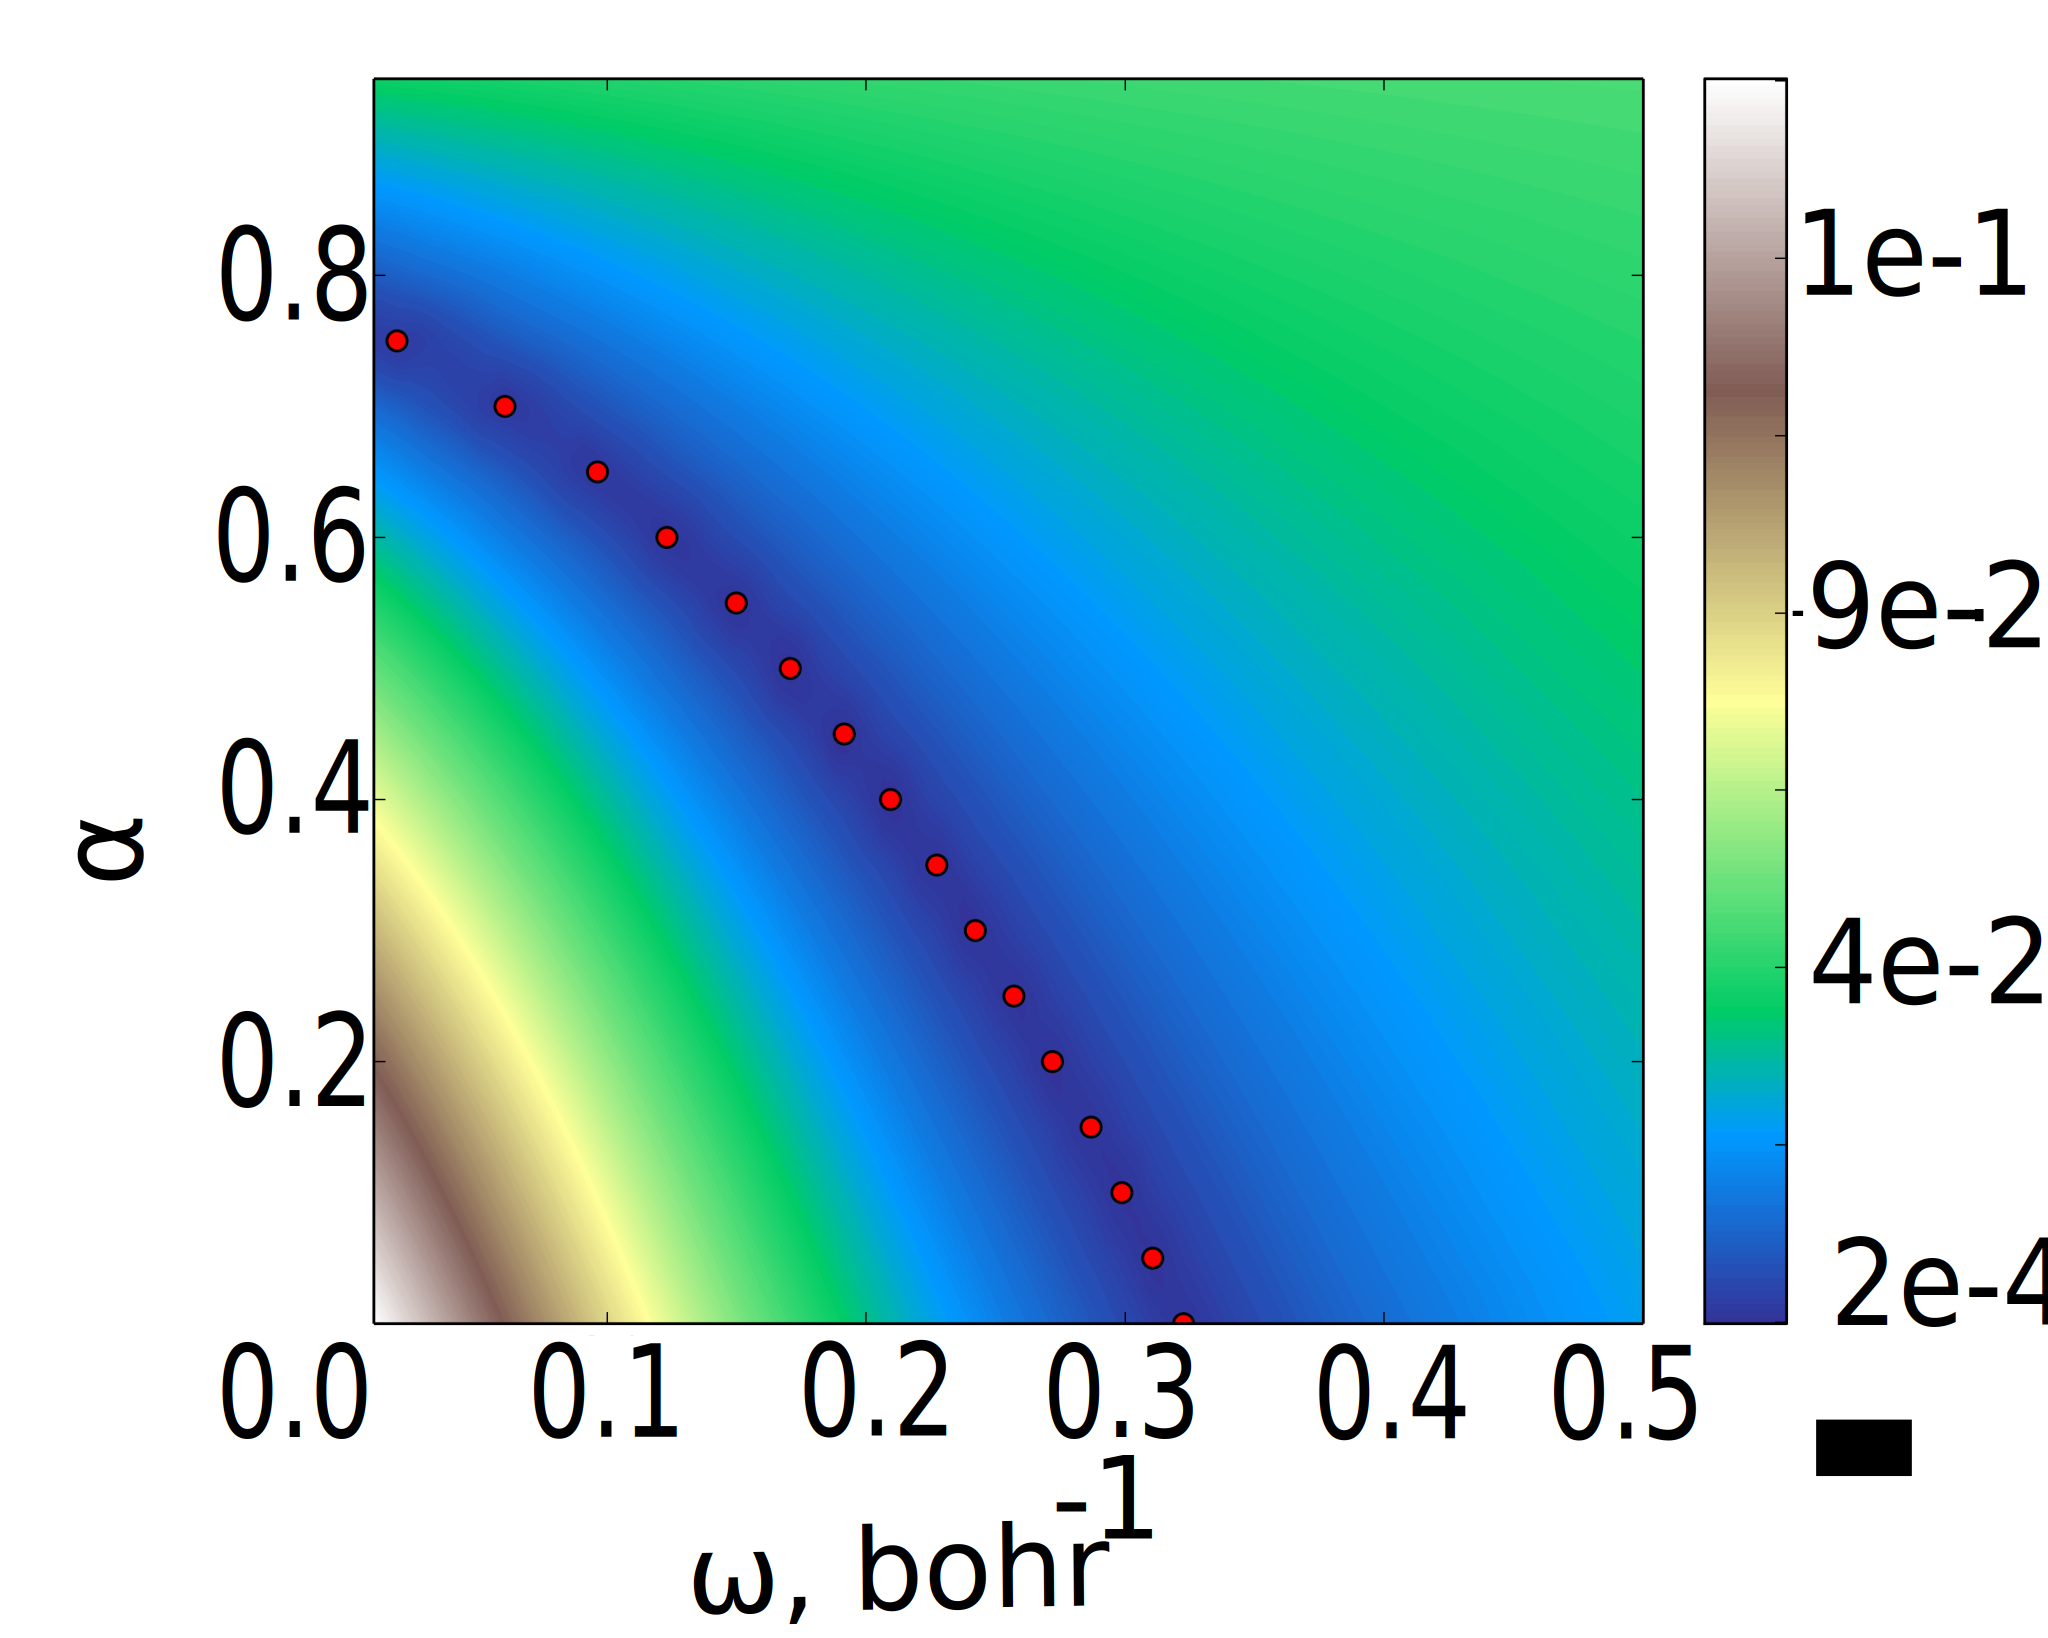
\includegraphics[width=0.5\textwidth]{Figures/Benzene/benzene2D}
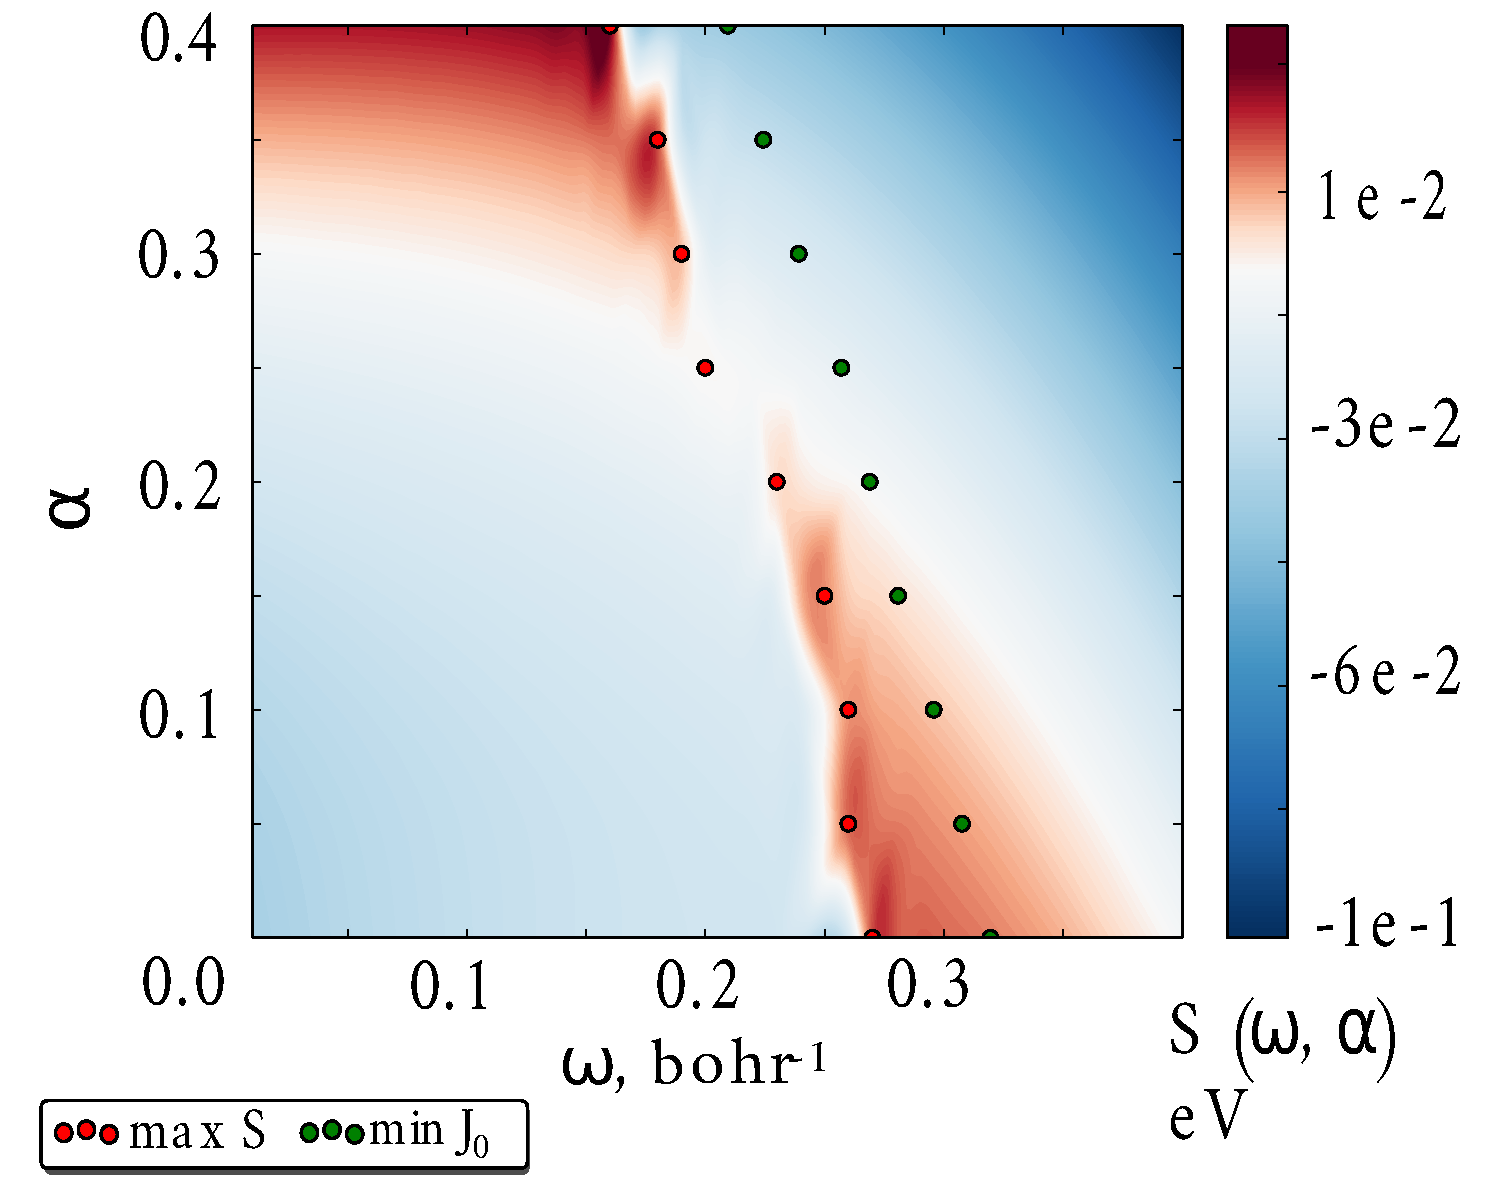
\includegraphics[width=0.5\textwidth]{Figures/Benzene/benzene_S_stab_ion_cut_all.pdf}
\caption{(left panel) $J(\alpha,\omega)$ for the case of benzene molecule. The valley of minimal $J(\alpha,\omega)$ is denoted with red dots. (right panel) Lowest eigenvalue of the stability matrix of benzene as function of $\alpha$ and $\omega$. }
\label{fig:Benzotrsh}
\end{figure}
Another important issue is the stability of the ground state solution to, \textit{e.g.}, change of the multiplicity (so called triplet stability). 
If the solution is not stable with this respect, the TDDFT procedure produces imaginary excitation energies.
A convenient way to estimate the stability is to look at the lowest eingenvalue of the 
matrix $\mat{A}$ in the Casida's equation (\ref{eq:casida}).
Its lowest eigenvalue corresponds to the transition from the HOMO to LUMO and thus should be real.
The stability is strongly dependent on the amount of the exact exchange and thus on the $\alpha$ and $\omega$ parameters.
The example for benzene molecule is shown in the right panel of Figure~\ref{fig:Benzotrsh}.
In general, the regions of highest stability do not coincide with minima of $J(\alpha,\omega)$.
Since stability issue is more crucial to obtain reliable results than self-interaction error, the values of $\alpha$ and $\omega$ in the stable domain should be preferred.
The LC-BLYP parameters for different systmes studied here are summarized in Table~\ref{tab:params}.

\begin{center}
\begin{table}[h]
\caption{Optimized OTRSH parameters for different systems studied in this thesis.}
\begin{tabular}{|l|l|l|}
\hline
System & $\alpha, [bohr^{-1}]$ & $\omega, [bohr^{-1}]$	\\
\hline
Li & 0.24 & 0.25 \\
\hline
CO$_2$ & 0.40 & 0.33 \\
\hline
C$_6$H$_6$ & 0.00 & 0.32 \\
\hline
\end{tabular}
\label{tab:params}
\end{table}
\end{center}
%In contrast to the behaviour of the $J$-functional \eq{eq:J_ao}, the lowest eigenvalue of the stability matrix has no such prototypical dependence on $\alpha$ and $\omega$ as the comparison of the right panel in Figure \ref{fig:Benzotrsh} with Figure \ref{fig:SulphurStab} shows where the respective HOMO-LUMO gap for the S$_8$-molecule is shown.
%Further, the choice of a particular set of parameters from the minimal parabola of the right panel of Figure \ref{fig:Benzotrsh} has a strong influence on the excitation energies and leads even to negative excitaiton energies for some molecules.
%Here, as a second criterion for the optimal parameters, the derivative discontinuity is chosen.
%\textcolor{blue}{figure}
%\textcolor{green}{How to indicate that the optimisation and cration of figures was not done by me?}
%The parameters resulting from this are $\alpha=0.00$ and $\omega=0.32$.

\subsection{Electrostatic Potential and Dyson orbitals}
\begin{wrapfigure}{L}{0.5\textwidth}
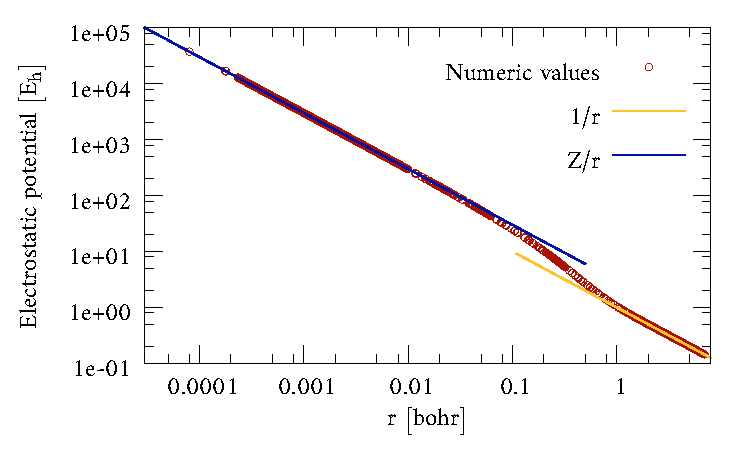
\includegraphics[width=0.5\textwidth]{Figures/ESP}
\caption{Double-logarithmic plot of the ground state ESP for Li$^+$ (red circles; $Z=3$), K$^+$ (blue circles; $Z=19$) and Xe$^+$ (green circles; $Z=54$) as a function of distance from the nucleus and its limiting cases at large ($1/r$) and small ($Z/r$) distances.}
\label{fig:esp}
\end{wrapfigure}
%Considering a state as linear combination of CI-states is denoted as weak-coupling representation \cite{McCarthy}.
The ESP used in this work is obtained with a modified version of \prog{NWChem} \cite{nwchem}, where the points at which this potential should be computed can be specified by the user.
Setting these points to the quadrature points of the integration scheme in the FEM calculations requires some extra effort but has the great advantage that no interpolation of the potential is required.
However, \prog{NWChem} can compute the values only up to a finite minimum distance to the nuclei due to numerical reasons.
The missing values are approximated as $Z/r$ where $Z$ is the respective nucleus charge and $r$ is the distance of the quadrature point to the closest nucleus.
Figure \ref{fig:esp} shows the quality of such an interpolation comparing the calculated ESP for three singly ionised systems with the two limiting cases at large and small distances from the nucleus.
It can be seen that the $\nicefrac{Z}{r}$ dependence approximates the ESP close to the nucleus very well.
An interpolation of the data on the complete domain in \prog{FreeWilly} \cite{FreeWilly} requires an scheme for scattered data such as RBF interpolation \cite{rbfSE,rbfInterpol,rbfSurf}, inverse distance interpolation \cite{adapt_idw,idw} or similar methods \cite{CompInterp,idw_krieging,interpol}.
However, these methods were found to be sensitive to the parameters and do not result in a smooth ESP due to spurious oscillations between the quadrature points.

The other external quantity needed to compute the intensities is the DO that is computed in the framework of this thesis with the in-house code \prog{DYSON} \cite{MAgg}.
The wave functions of the initial $|\Psi^N\rangle$ and final $|\Psi^{N-1}\rangle$ states are computed with the \prog{NWChem}-code which is modified to produce more verbose output to be able to reconstruct the molecular orbitals.
As quantum-chemical method, the previously described Tamm-Dancoff approximation to (TD)DFT method with the OTRSH LC-BLYP \cite{lcBLYP} functional and the def2-TZVP \cite{def2tzvp} basis set are used.
The respective data are extracted and reformatted with a self-written script \cite{nwc2dy}, creating the input for \prog{DYSON}.

The Kohn-Sham orbitals (obtained by ground state DFT) and CI-coefficients (obtained by linear-response TDDFT) as well as the atomic overlap matrix are interfaced to the in-house software \prog{DYSON} \cite{MAgg} (G.Grell) that computes the DOs.
Throughout this work, the initial state is chosen to be the ground state of the respective neutral $N$-electron system that is represented with one slater determinant $|\Psi_j^N\rangle$ whereas the final state can be the ground or excited state of the ion, having the general CI-expansion \eq{eq:excCI}.

Thus, the DO can be written as
\begin{equation} \label{eq:doCI}
|\Psi^\text{DO}\rangle=\sum_{ia} c_{ia} \langle \Psi_j^N| \Psi_{ia}^{N-1} \rangle.
\end{equation}
%Knowing the overlap matrix of the atomic orbitals, the overlap integral \eq{eq:doCI} is reduced to a summation of the transition coefficients $c_{ja}$ \cite{MAgg} which are obtained as eigenvectors of the Casida equation \eq{eq:casida}.

\section{Free Electron Function}
\label{sec:grid}
The main goal of this thesis is the development of a FEF representation using a finite element scheme that is implemented the program \prog{FreeWilly} \cite{FreeWilly}.
It is based on the library \prog{Libmesh} \cite{libmesh} which itself uses several libraries for the required linear algebra \cite{petsc, slepc1,eigen} and the mesh-setup \cite{tetgen,qhull}.
As discussed in section \ref{ch:fem}, the most crucial step in a FEM simulation is the setup of the grid.
The \prog{FreeWilly}-code implements several closely related schemes, with are described in section \ref{ch:GridSetup.}.
Moreover, for comparison purposes here plane wave functions written in a truncated Coulomb basis are used to estimate the PES intensities in the DO formalism.
This method has shown to yield good agreement with experiment for various molecules \cite{ezDyson,GrellKuehn,DO_TDDFT}.

\subsection{Coulomb Waves}
%TODO Make the explanation of the grids more clear
An established representation of the FEF in the Dyson formalism is the expansion of a plane wave in Coulomb wave functions \cite{ezDyson,do_modCoul,DO_TDDFT}.
Such an approach is used here for comparison with the results obtained using a photoelectron function as computed with an finite element/infinite element method.
The results using a Coulomb wave as FEF are obtained by the \prog{ezDyson} v. 3.0 \cite{ezDyson} program in which integration of the dipole transition moment \eq{eq:sigma_do} is performed using a uniform cubic grid.
The particular parameters for these grids are chosen such that they are converged to avoid a significant influence due to integration errors.
In particular, for the atomic lithium here a cubic box with a diameter of $4\,$\AA\, and $160$ grid points is chosen.
For carbondioxide, the grid was choosen to be $8\,$\AA\,  along the molecular axis and $8\,$\AA,\ with $360$ and $200$ grid points respectively.
The grid for benzene has a height (orthogonal to the molecular plane) of $8\,$\AA\, and a diameter of $12$\AA\, in both directions of the molecular plane with $380$ points in each direction.
To reduce the computational effort, moreover, all transitions for which the norm of the corresponding DO is below \textcolor{red}{$...$ Where do I find this number?} are neglected.

\subsection{Setup of the Grid}
\label{ch:GridSetup}
%The most crucial part in a FEM simulation is the mesh being used. 
In the program \prog{FreeWilly}, the finite elements are constructed using a set of points via Delaunay triangulation %TODO (see \ref{app:delaunay} for details) 
with the library \prog{tetgen} \cite{tetgen}.
The distribution of these points is responsible for the quality of the obtained solution via many parameters in a non-trivial way.
%It is expected that the most important of these parameters are
While choosing these parameters one should account for:
\begin{itemize}
   \item \textbf{The molecular geometry} The grid point density should be large close to the atomic nuclei and coarser at larger distances.
   \item \textbf{The kinetic energy} (wavelength of the outgoing wave) of the photoelectron which determines the maximum distance between two grid points
   \item \textbf{The largest angular momentum of the Dyson orbital} determines the largest angular momentum of the photoelectron to be resembled assuming that the dipole selection rules $\Delta l=\pm 1$ hold.
   This is in general not strictly true but can be used to approximately estimate the non-zero contributions to the intensity.
\end{itemize}

To account for these properties in the best way, here two algorithms are used, based on a scheme suggested by Son and Chu \cite{Son_Chu} but using different functions for the distribution of points.
In this scheme, the molecular region is composed of spheres with different radii, centred at the nuclei and whose overlapping regions belonging to different atoms are cut off.
%Thus, the setup of a point distribution is subdivided into three parameters to be found: The radii of the individual spheres, the distribution of points on these spheres and the number of points per sphere.
%In this work the point-distribution is chosen similarly to the grid used by Son and Chu \cite{Son_Chu} which is based on spherical distributions around the atoms whose overlapping regions are cut off.

To yield a reasonable mesh, the maximal radii $r_\text{max}$ of these spheres need to be larger than the bond lengths to avoid disjoint simulation domains in molecules.
Using such a scheme, the global grid is determined by the size of the largest sphere $r_\text{max}$, the number $N$ of spheres being used for each atom as well as the distribution of the radii of spheres and angular distributions of points on each sphere, respectively.
For the radius of $i$th sphere, Son and Chu \cite{Son_Chu0} suggested the following scheme
\begin{equation} \label{eq:son_map}
r_i=\frac{iq}{N-i+\frac{qN}{r_\text{max}}} \qquad i=1,\hdots ,N,
\end{equation}
where $q$ is a parameter that determines the distance between the most inner spheres.
Using this function, the smallest spheres ($i<<N$) are scaled linearly, having distances $r_\text{max}/N$ between the closest spheres.
The radii of the largest spheres depends non-trivially on the parameters but can become very large if $q$ is small.
In the limit of infinitely large $q$, \eq{eq:son_map} corresponds to a uniform distribution of spheres.

To obtain better control of the distances between the inner spheres and the maximum distance which needs to be consiberably smaller than the wave length, the formula
\begin{equation} \label{eq:tm_map}
r_i=\frac{iq}{\left( \frac Ni \right)^s \left(\frac{Nq}{r_\text{max}}-1\right) +1} \qquad i=1,\hdots ,N 
\end{equation}
is suggested in this work.
It has two degrees of freedom $q$ and $s\geq 1$, where the condition $N>\frac{r_\text{max}}{q}$ needs to be fulfilled to ensure positive radii.
Here $q$ is the asymptotic distance between two spheres, whereas the distance of inner spheres can be tuned by the power $s+1$ so that the inner spheres become very dense.
%Thereby it is important to mention that in this scheme (in contrast to the above one) the (asymptotic for $r\rightarrow \infty$) maximum distance between two spheres is $l$ and hence could be physically chosen to $l\approx \frac \lambda 2$.

%While the distribution of spheres follows, at least on a qualitative level, a clear scheme since it should always resemble the local kinetic energy, the distribution of points on the surface of each sphere more complicated.
%Here, a regular distribution is a good choice, but on the non-linear topology of the sphere, regularity is in general more challenging.
In addition to a radial distribution that resembles the radial structure of the wave function, also a proper angular distribution of the points is required.
The problem of distributing points regularly on a sphere is non-trivial.
%Depending on the measure being used, several schemes are proposed.
A popular choice in earth sciences are so-called geodesic grids \cite{geodesic1,geodesic2,geodes_charge}, but their construction allows only for exponentially growing mesh-sizes and thus they are not of interest here.
Instead, in the implemented protocol several point-sets stemming from quadrature rules of numerical integration schemes of a given order on a sphere are used.
The order in these schemes corresponds to the largest spherical harmonic that can be exactly integrated, leading to Lebedev-grids \cite{lebedev,lebedev2} and spherical t-designs \cite{t-design1, t-design2}.
These distributions are found more often in quantum-chemical contexts \cite{LebQC1,LebQC2,lebDFT,lebDFT2} and will be used in this thesis.
Further, several point-sets implemented in \prog{FreeWilly} represent point distributions corresponding to extrema of certain quantities such as the minimum of the Riesz s-energy\cite{fliegeMaier} or other geometric properties \cite{womersley,wom2,wom3}.
%The computation of the above-mentioned point-sets is very demanding to compute and thus are hard-coded in the current implementation.
For comparison, finally also the spherical Fibonacci mapping \cite{fibonacci,fibonacci2} is implemented.
It yields a less regular point-distribution but is computationally much easier to obtain and, in contrast to the distributions discribed above, can be defined for any number of points.
\begin{figure}
   %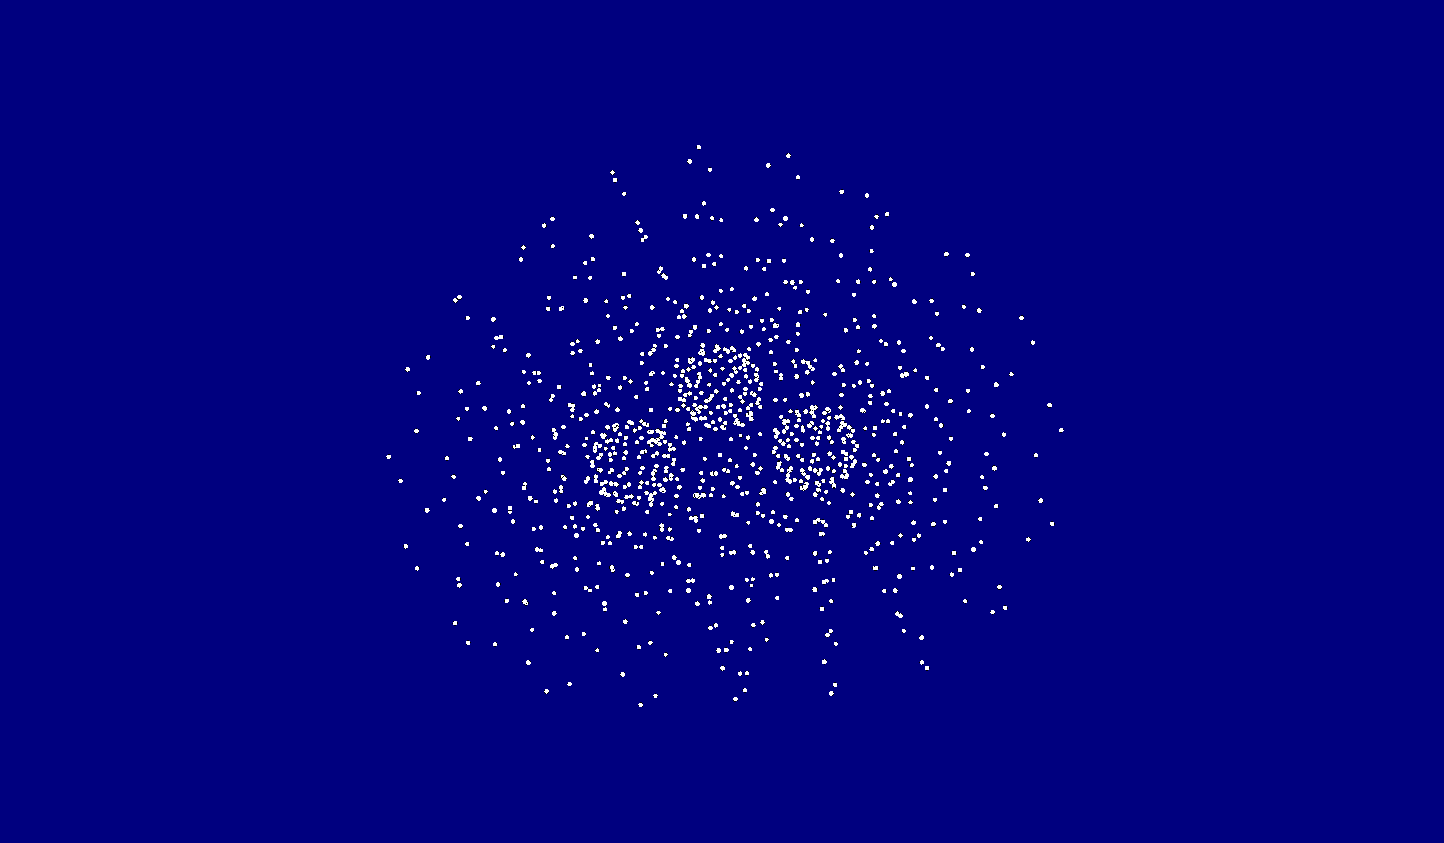
\includegraphics[width=0.5\textwidth]{water1}
   %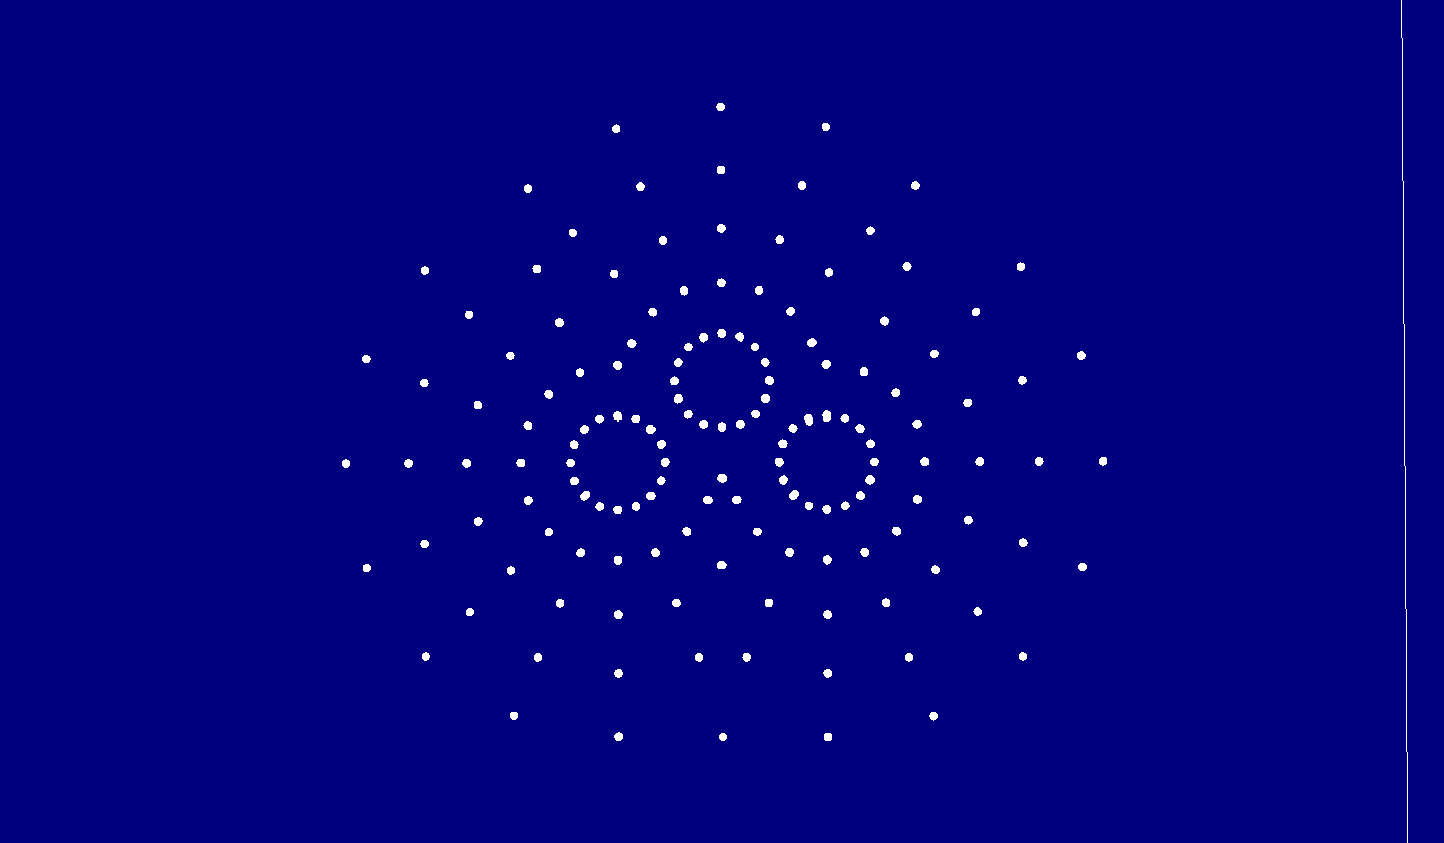
\includegraphics[width=0.5\textwidth]{water2}
   %\caption{Example of a mesh for the water-geometry. It consists of $5$ spheres with constant number of points per sphere. The overlapping regions are cut off. Left: cut through the nuclear plane. 
   %\textcolor{red}{add figure with distribution: tm}}
   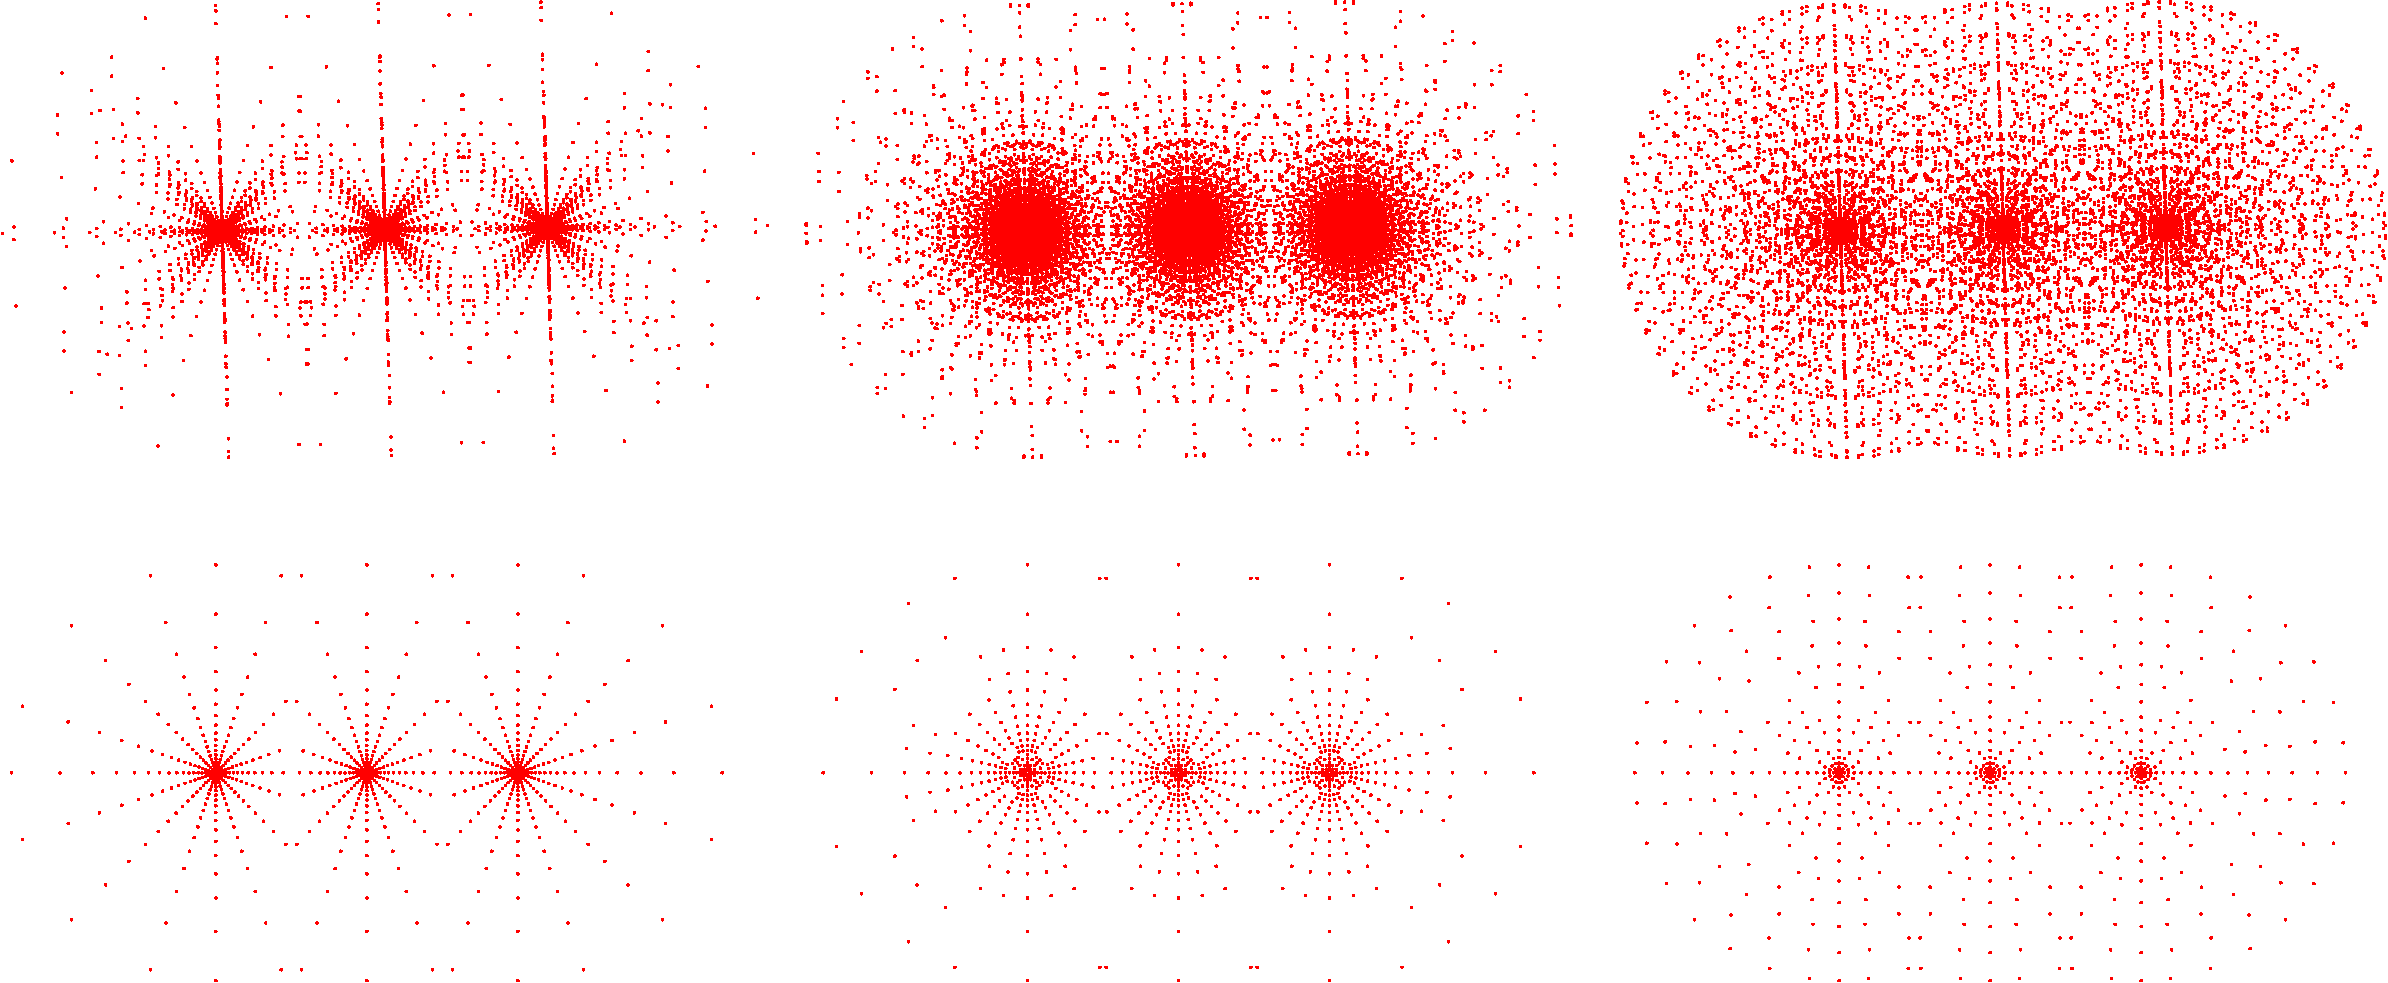
\includegraphics[width=\textwidth]{Figures/CO2_grid}
   \caption{Examples of point-distributions for a CO$_2$-molecule with $r_\text{max}=3\,$a.u. and $N=18$ spheres, in the upper row the full mesh and in the lower row the cuts through the molecular plane are presented.
   (left panel) constant number of points $M$ per sphere, radial scheme \eq{eq:son_map} with $q=0.7$; (central panel) radial scheme \eq{eq:son_map} with number of points according to \eq{eq:son_num} with $q=0.7$; (right panel) radial distribution from \eq{eq:tm_map} with $q=0.7$, $s=2$ and number of points per sphere according to \eq{eq:tm_num}}
   \label{fig:molmesh}
\end{figure}
However, since in finite element theory the simulation box neither needs to be really round nor is there any global functional defined on it, the quality of a particular distribution might be not critical here.
%Some explanations are given here:\\ %https://www.maths.unsw.edu.au/about/distributing-points-sphere
%Approach used for climate models: so-called geodesic grids: subdivision of polyhedra, projected onto the sphere\cite{geodesic1, geodesic2}, see also
%http://kiwi.atmos.colostate.edu/BUGS/geodesic/
%http://kiwi.atmos.colostate.edu/BUGS/pdf/ZM-grid.pdf
%http://kiwi.atmos.colostate.edu/BUGS/pdf/conservation.pdf
%http://kiwi.atmos.colostate.edu/BUGS/pdf/ccsr.pdf

%Whether the approach of subdividing the atomic meshes into radial and angular parts as opposed to another volume tessellation can be questioned and may turn out to be inefficient.
%Application of Geodesic grid in calculating surface charges: \cite{geodes_charge}, also mentioning Connolly algorithm (refs 26, 29 therein).

%The second scheme has a divergence around $Nq=r_\text{max}$. 
%It can be shown that the condition $N\leq \frac rq $ is enough here to stabilise it.

%\textcolor{yellow}{
%If the above described procedures prove to be too inefficient, one could try to implement some WKB-based scheme similar to \cite{impLDVR} but in 3D.
%Thereby, the number of points in a given volume element is determined by $N_i=\frac{\alpha_i}{\alpha} N$ where $\alpha=\sum_i \alpha_i $ and
%\[ \alpha_i= \int_V dV \sqrt{2\mu (E-V(r))} \]
%.This ensures dense points there, where the potential is lowest and a coarse mesh far away; however, a consistent formulation in 3D would need to be invented.
%}
%
%To account for the molecular geometry and the general tendency of the photo electron to oscillate stronger in the vicinity of the nuclei, the mesh is built out of spheres, centred at the nuclear positions.
%Thereby, a study of Son \cite{Son_Chu0} had shown that it is numerically most efficient when the overlapping regions of these spheres are cut out.
%Figure \ref{fig:molmesh} shows an example for the water molecule.
%
%For the radial distribution we will use the the function
%\begin{equation}
%r_i = \frac{1+x_i}{1-x_i+\frac{2L}{r_{max}}} L \qquad x_i = \frac{2i}{N_r} -1
%\end{equation}
%suggested by Son \textit{et. al.}\cite{Son_Chu0, Son_Chu}.
%The parameters $N_r$, $L$ specifying the number of spheres and their distribution; the larger $L$ is, the denser are the spheres close to the centre.
%
%The optimal choice of these parameters as well as the angular distribution of points on the spheres is still an open question.
%Finally, after putting the points together as described above, they are connected to a Delaunay triangulation using \prog{tetgen} \cite{tetgen}. 
%Here additional points may be introduced to guarantee well-shaped elements (\texttt{i.e.} no sharp peaks).
%
%One scheme suggested by Son and Chu \cite{Son_Chu0}:
%\begin{equation} \label{eq:son_map}
%r_i=\frac{il}{N-i+\frac{lN}{r_\text{max}}} \qquad i=1,\hdots ,N 
%\end{equation}
%where $l$ is a parameter to chose.
%Own scheme:
%\begin{equation} \label{eq:tm_map}
%r_i=\frac{il}{\left( \frac Ni \right)^p \left(\frac{Nl}{r_\text{max}}-1\right) +1} \qquad i=1,\hdots ,N 
%\end{equation}
%where $l$ and $p\leq 1$ are parameters to chose. Thereby it is important to mention that in this scheme (in contrast to the above one) the (asymptotic for $r\rightarrow \infty$) maximum distance between two spheres is $l$ and hence could be physically chosen to $l\approx \frac \lambda 2$.
%
%The second scheme has a divergence around $Nq=r_\text{max}$. 
%It can be shown that the condition $N\leq \frac rl $ is enough here to stabilise it.
Finally, not only the scheme used to distribute the points on the spheres, but also the number of points to be distributed is of importance.
In \cite{Son_Chu0}, the number of points $M$ for each sphere is chosen to be a constant parameter.
Application of such a scheme is shown in Figure \ref{fig:molmesh} in the left panel.
However, it can be seen that this leads to unbalanced distances between radial and angular neighbours.
%Besides a constant number, also a constant spherical density (hence $M\propto r^2$) is possible.
%However, it might be sensible to follow a similar idea than in the radial mapping: Being fine close to the nuclei and get coarser with increasing distance.
To obtain a more regular mesh, for which the radial distances between points are comparable to the distances along the sphere, here for both radial distributions, \eq{eq:son_map} and \eq{eq:tm_map}, the criterion $d_\text{spheric}=\sqrt{\frac{4\pi r_i^2}{M_i}}\approx r_i-r_{i-1}$ is used, where $d_\text{spheric}$ is the average distance between two points on the sphere $i$.
For the above described radial schemes, this results in 
\begin{equation}\label{eq:tm_num}
M_i= \frac{4\pi}{ \left(1-\frac{i-1 }{i}\frac{N-i+\frac{lN}{r_\text{max}}}{N-i+1+\frac{lN}{r_\text{max}}}\right)^2 }
\end{equation}
for the first scheme, denoted as \textit{son} in the following, and 
\begin{equation} \label{eq:son_num}
M_i= \frac{4\pi}{\left(1-\frac{i-1 }{i}\frac{ (\frac{N}{i})^p \left(\frac{lN}{r_\text{max}}-1\right)+1}{ (\frac{N}{i-1})^p\left( \frac{Nl}{r_\text{max}} -1 \right) +1 } \right)^2 }
\end{equation}
for the radial mapping \eq{eq:tm_map} which will be referred to as \textit{tm}.
%Since some of the spherical schemes described above allow only for certain numbers of points each, here, the best approximation is used respectively.
%Special mapping schemes are the constant radial mapping $r_i=a i$ which corresponds to a constant spherical grid density $N_i=4\pi a^2 i^2$ and an exponential map $r_i=q^i r_0$ which would require a constant number of spherical grid points $N_i=\frac{4\pi q^2}{(1-q)^2}$ according to the rule derived above.

Using this procedure, the mesh is determined by the molecular geometry the largest radius $r_\text{max}$, the radial distribution (\textit{son} or \textit{tm} with parameters $s$ and $q$) and the angular point distribution.
%TODO From here on I could not completely follow what you wanted to say.
Importantly, the number of points per sphere is fixed and is illustrated in the Figure \ref{fig:maps} b) for a given set of parameters.
\begin{figure}[h]
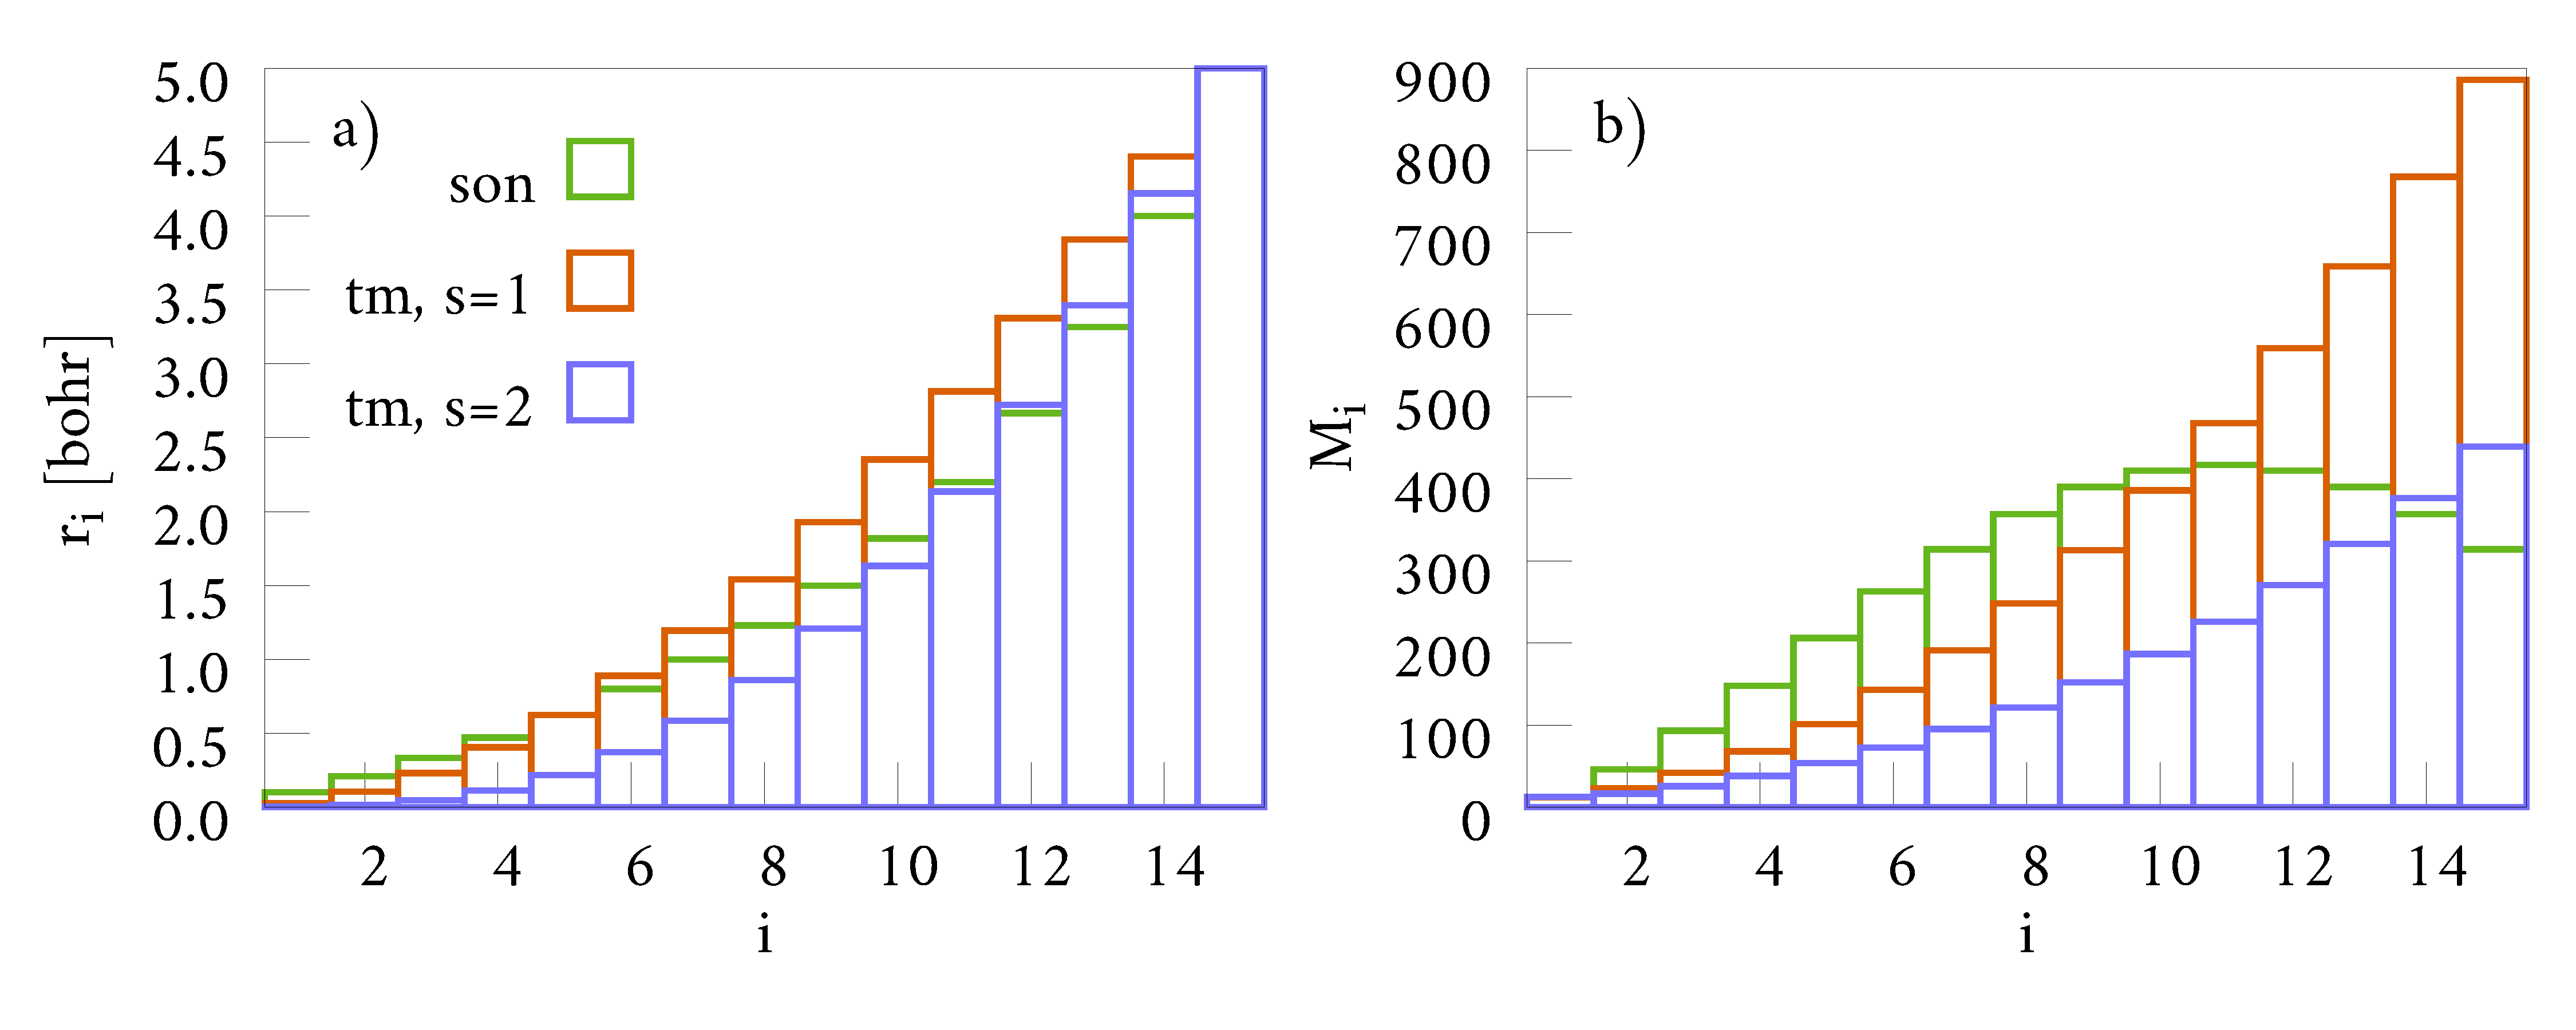
\includegraphics[width=\textwidth]{Data/radial_mapping}
\caption{Comparison of the radius (left) and number of points (right) of the $i$. sphere using $N=15$, $r_\text{max}=5$ and $q=2$.
The radial scheme son corresponds to \eq{eq:son_map} and  tm to \eq{eq:tm_map}.
For the number of points per sphere, the \eq{eq:son_num} and \eq{eq:tm_num} are used, respectively.}
\label{fig:maps}
\end{figure}
Figure \ref{fig:maps} a) shows the size of the radii of the individual spheres which follow in all three cases a similar scheme.
It is important to note therein that the parameter $q$ has a different interpretation in the different radial schemes and thus a direct comparison of the son and tm-schemes is not possible.
In contrast to the distribution of radii, the number of points $M$ on sphere number $i$ is qualitatively different for the different radial distributions as Figure \ref{fig:maps} illustrates. 
Here, especially the decay of $M$ for the largest spheres in the son-scheme should be noted which is an indication that this function is not well-suited for the representation of a FEF.

Numerical tests on these schemes show, however, that the different schemes introduced above lead to finite element meshes of similar quality (see section \ref{app:CompSetup}).
The tests presented in the following are done on a single atom using a box-size of $r_\text{max}=7\,$bohr and $N=20$ spheres.
As radial distribution, the tm-mapping \eq{eq:tm_map} is used for the schemes denoted as \textit{const} and \textit{tm} whereas \eq{eq:son_map}) map is used for the scheme \textit{son}.
The number of points per sphere is $M_i=74$ for all spheres for the \textit{const} scheme and according to \eq{eq:tm_num} and \eq{eq:son_num} for the others, respectively.
The parameters for the radial mapping are chosen as $q=1.8$ and $s=2.6$.
In Figure \ref{fig:SchemHist}, the distribution of the ratio of the longest edge to the height of the smallest side is shown, similar graphs for further quantities indicating the quality of the tetrahedra are given in \ref{appFig:SchemHist} in supplement and show a very similar behaviour.
Thus, the quality of the generated tetrahedra is very similar for the three schemes which is, in parts, due to the modifications applied by \prog{tetgen} but can be moreover explained by the adaptive number of gridpoints per sphere according to \eq{eq:tm_num} and \eq{eq:son_num} which ensures some regularity of the point distribution.
\begin{wrapfigure}{R}{0.5\textwidth}
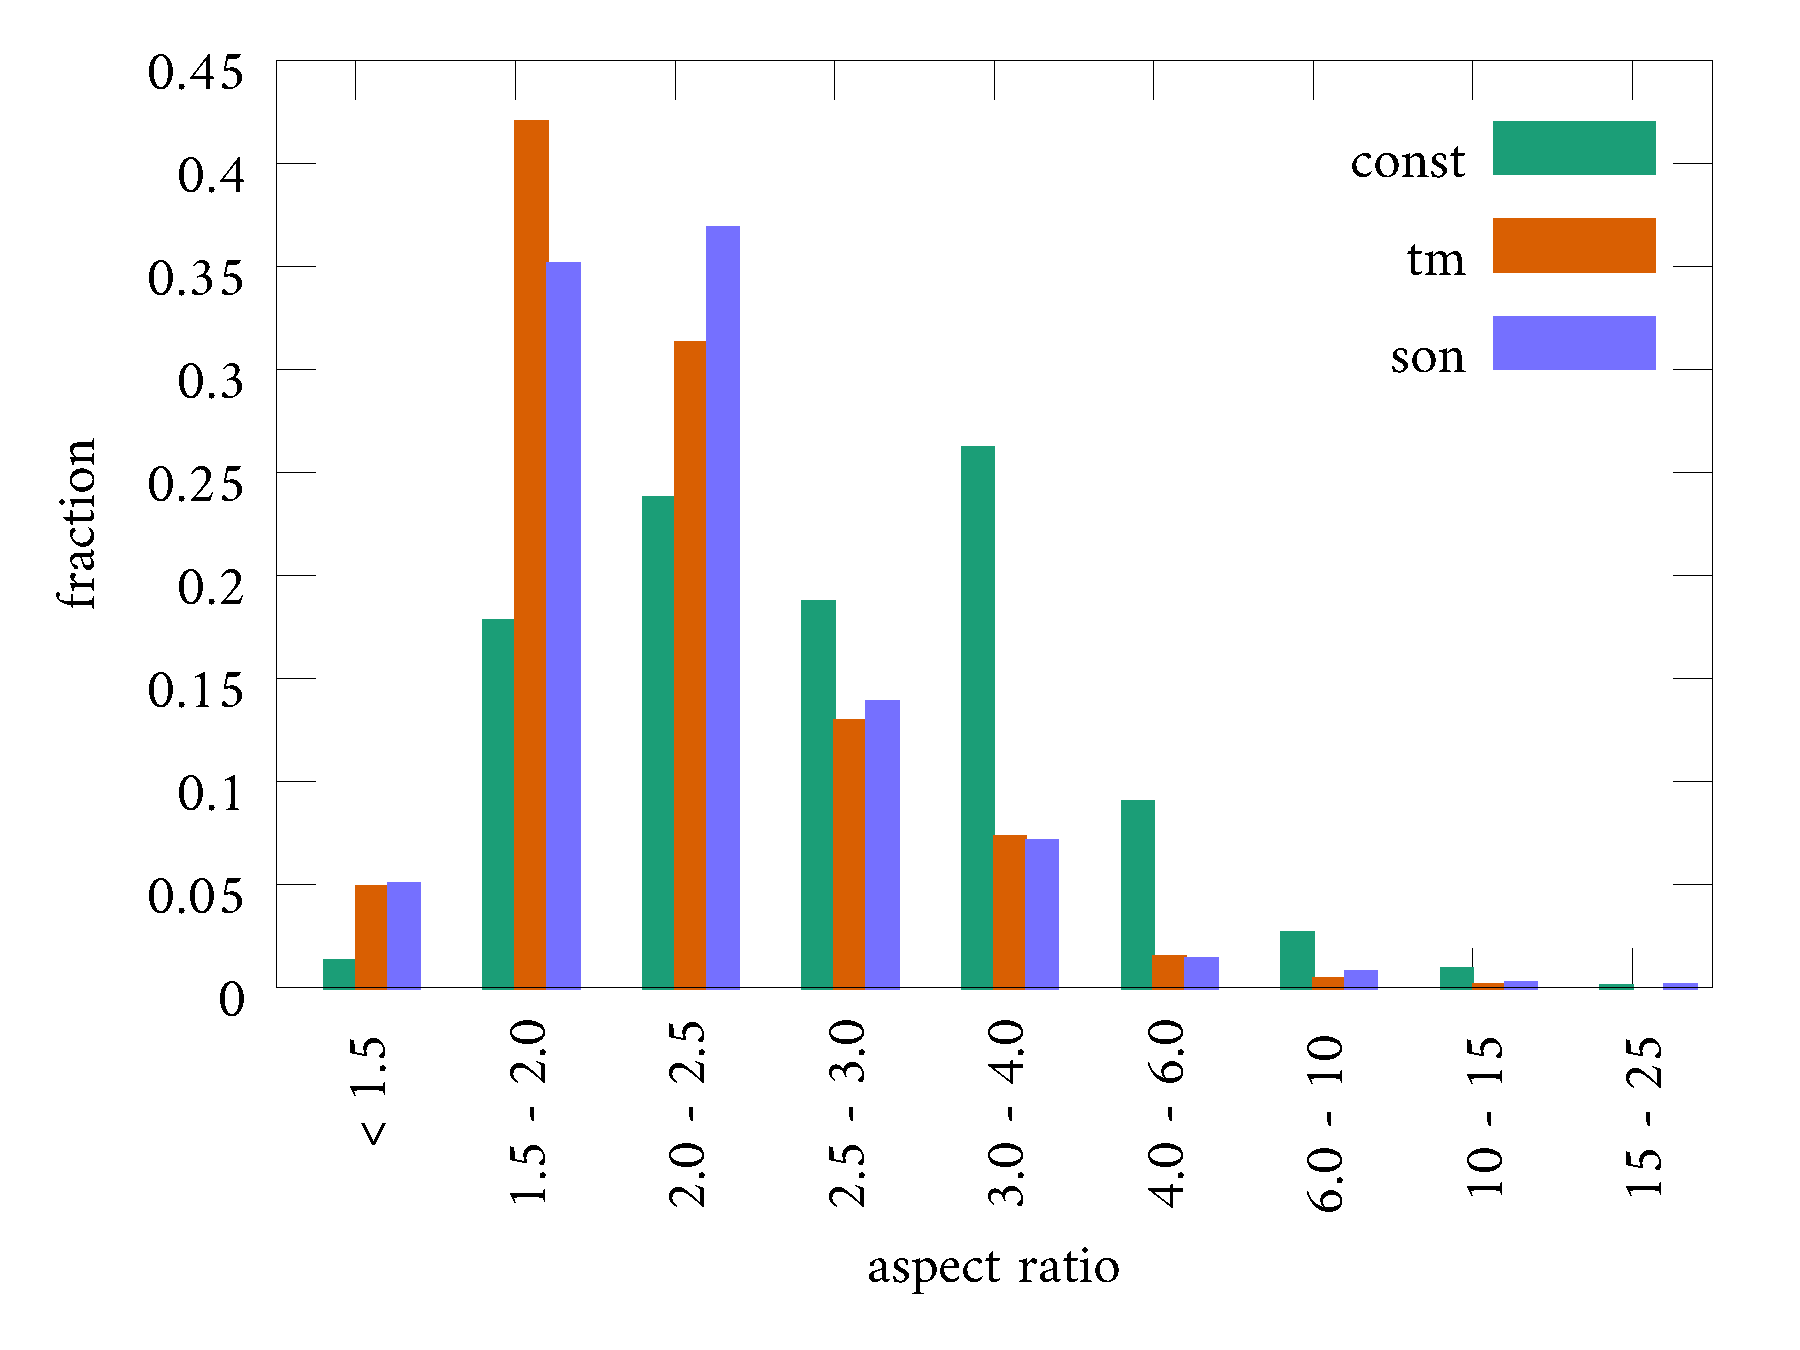
\includegraphics[width=0.49\textwidth]{Figures/Radi_hist.pdf}
\caption{Distribution of aspect ratio (longest edge length divided by the smallest side height).
   Be aware that the ranges of the different bins differ.}
\label{fig:SchemHist}
\end{wrapfigure}
In this work, unless specified, the tm-scheme is used in the following since it provides more control about the distances between the outer region and thus is better suited for the description of FEFs.
Similar studies are done for the properties of the solutions obtained using the different spherical grids introduced above which are shown in section \ref{appCompSetup}.
However, the results show only minor differences between the different schemes.
In this work unless otherwise noted, the Lebedev scheme is used which provided a higher density of states (DOS) than the other schemes in this test.
